\documentclass{article}
\usepackage[margin=1in]{geometry}
\usepackage{amsmath,amsthm,amssymb}
\usepackage{bbm,enumerate,mathtools}
\usepackage{tikz,pgfplots}
\usepackage{chessboard}
\usepackage[hidelinks]{hyperref}
\usepackage{multicol} % Problem 35

\newenvironment{question}{\begin{trivlist}\item[\textbf{Question.}]}{\end{trivlist}}
\newenvironment{note}{\begin{trivlist}\item[\textbf{Note.}]}{\end{trivlist}}
\newenvironment{references}{\begin{trivlist}\item[\textbf{References.}]}{\end{trivlist}}
\newenvironment{related}{\begin{trivlist}\item[\textbf{Related.}]\end{trivlist}\begin{enumerate}}{\end{enumerate}}


\begin{document}

\rating{3}{3}
In geometry, a deltahedron is a polyhedron whose faces are all equilateral triangles.

\begin{figure}[ht!]
  \centering
  % Graphics3D[
  %   {
  %     Opacity[0.75],
  %     EdgeForm[{Thick, Blue}],
  %     Glow[White],
  %     PolyhedronData["Octahedron", "GraphicsComplex"]
  %   },
  %   Boxed -> False
  % ]
  \raisebox{-0.5\height}{
    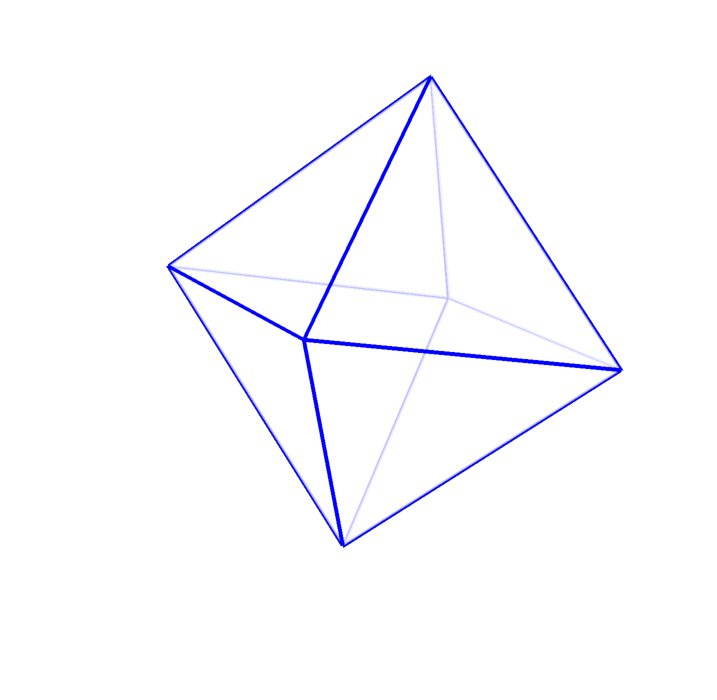
\includegraphics[scale=0.8, trim=80 70 45 35]{assets/deltahedra/octahedron.pdf}
  }
  % Graphics3D[{
  %     Opacity[0.75],
  %     EdgeForm[{Thick, Blue}],
  %     Glow[White],
  %     Tetrahedron[{
  %       {1, 0, -1/Sqrt[2]},
  %       {-1, 0, -1/Sqrt[2]},
  %       {0, 1, 1/Sqrt[2]},
  %       {0, -1, 1/Sqrt[2]}
  %     }],
  %     Tetrahedron[{
  %       {1, 0, -1/Sqrt[2]},
  %       {5/3, 0, 5*Sqrt[2]/6},
  %       {0, 1, 1/Sqrt[2]},
  %       {0, -1, 1/Sqrt[2]}
  %     }],
  %     Tetrahedron[{
  %       {-1, 0, -1/Sqrt[2]},
  %       {-5/3, 0, 5*Sqrt[2]/6},
  %       {0, 1, 1/Sqrt[2]},
  %       {0, -1, 1/Sqrt[2]}
  %     }]
  %   }, Boxed -> False]
  \raisebox{-0.5\height}{
    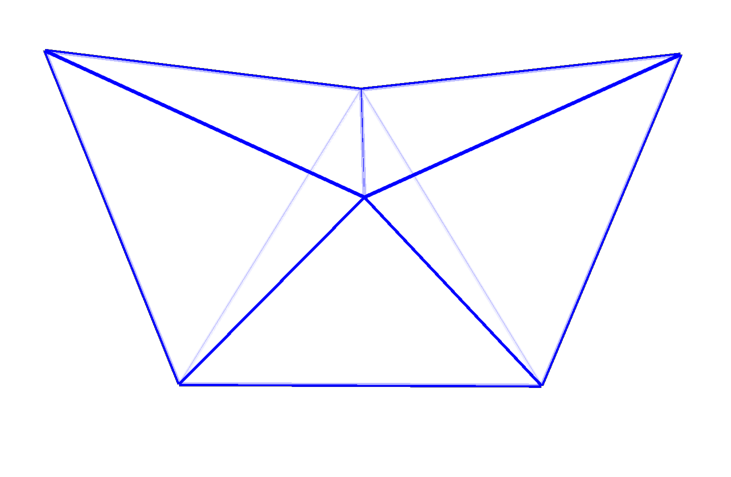
\includegraphics[scale=0.8, trim=25 40 28 25]{assets/deltahedra/biaugmented_tetrahedron.pdf}
  }
  \caption{The two deltahedra consisting of eight triangles: the octahedron and the biaugmented tetrahedron.}
\end{figure}

\begin{question}
  How many polytopes can you make out of $n$ equilateral triangles?
\end{question}

\begin{related}
  \item What if none of the adjacent faces can be coplanar?
    (e.g. the ``scaled-up'' tetrahedron is not allowed)
  \item How many with some sort of symmetry?
  \item What if squares or pentagons are used instead?
  \item What if pentagons and triangles are used?
  \item How does this generalize to higher dimensions?
  \item Which $n$-cell nets can produce the greatest number of distinct polytopes?
  \item How many $n$-cell nets can form at least one polytope?
\end{related}

\begin{references}
  \item \url{https://en.wikipedia.org/wiki/Deltahedron}
\end{references}

\begin{note} ~ \\
  The tetrahedron is the only deltahedron with $4$ faces.\\
  The triangular bipyramid is the only deltahedron with $6$ faces.\\
  There are at least five examples of deltahedra with $10$ faces:
  the pentagonal dipyramid,
  the augmented octahedron,
  and the three ways to augment the biaugmented tetrahedron.
\end{note}

\end{document}
